\subsection{Základní datové struktury}
V programu jsou často využívány datové struktury zásobník (struktura \verb|stack_type|, soubory \verb|stack.c/.h|) a již zmíněný vektor (struktura \verb|vector_type|, soubory \verb|vector.c/.h|).
V průběhu programu bude také nutné převést data z vektoru do zásobníku. Funkce převedení je v souboru \verb|conversion.c/.h|. Vzhledem k tomu, že se jedná o běžné datové struktury, nebudeme je podrobně popisovat. Zmíněné soubory jsou umístěny samostatně ve složce \verb|data_structures|. 

\subsection{Struktura pro reprezentaci čísel}\label{subsection:mpt}
Struktura pro reprezentaci `nekonečně' velkých čísel (struktura \verb|mpt|, soubory \\ \verb|multiple_precision_type.c/.h|) je pouze obalovací strukturou pro vektor integerů (dále označovány jako segmenty), jehož velikost se dynamicky realokuje podle potřeby.

Veškeré soubory týkající se struktury \verb|mpt| a práce s ní se nacházejí ve stejnojmenné složce \verb|mpt|.

Při vytvoření instance \verb|mpt| (funkcí \verb|mpt_allocate|) do vektoru přidáme jediný segment se zadanou číselnou hodnotou v rozsahu datového typu \verb|int|. Pro získání vyšších, resp.~nižších, čísel je zapotřebí přidat do vektoru další segmenty a v nich nastavit příslušné bity (funkce \verb|mpt_set_bit_to|). Každý $i$-tý prvek ve vektoru odpovídá $i$-tému segmentu čísla. Nultý segment má váhu nejmenší a s každým dalším segmentem se váha zvyšuje.

Je nutné počítat s tím, že čísla reprezentujeme dvojkovým doplňkem. \\Např.~číslo $2^{32}$\verb| = |0b11\dots 11 se sice vejde do jednoho segmentu, ale ve dvojkovém doplňku je rovno \verb|-1|, a proto je nutné přidat navíc segment samých nul, aby hodnota odpovídala $2^{32}$.

Vezmeme-li v potaz, že bity indexujeme v rozsahu \verb|size_t|, a budeme-li předpokládat, že program běží na 64-bitovém stroji, vidíme, že jedno číslo \verb|mpt| může mít až $2^{64}$ bitů a mít tedy hodnotu v rozsahu $\langle-2^{(2^{63})}, 2^{(2^{63})}-1\rangle$. Jedná se o čísla, která mají v dekadické soustavě přibližně $2,8\cdot{}10^{18}$ číslic. Nedokážeme tedy reprezentovat `nekonečně velká' čísla, na druhou stranu jsou tato čísla tak velká, že bychom na výsledky operací s nimi čekali příliš dlouho.

\subsection{Matematické operace s MPT}\label{subsection:mpt_operace}
Funkce pro matematické operace s instancemi \verb|mpt| se nachází v souborech \\\verb|multiple_precision_operations.c/.h|.

U všech operací je výsledná hodnota vrácena odpovídající funkcí jako ukazatel na novou instanci \verb|mpt|, nebo NULL když nastane chyba nebo nelze operaci provést se zadanými hodnotami. Vstupní operandy zůstávají nezměněné. Na konci každé operace by měla výsledná hodnota vždy být optimalizovaná funkcí \verb|mpt_optimize| tak, aby měla co nejmenší počet segmentů. 

Pro některé operace bylo zapotřebí vytvořit navíc operace absolutní hodnoty (funkce \\ \verb|mpt_abs|) a bitového posunu (funkce \verb|mpt_shift|).

Sčítání provádíme po segmentech a stav příznakového bitu \verb|CARRY| zjišťujeme funkcí \\\verb|addition_carry_|. Při sčítání musíme pro obecnou správnost výpočtu sečíst tolik segmentů, kolik má operand s nejvíce segmenty a poté ještě jeden segment navíc, kdyby došlo k nastavení MSB.

Základní princip implementovaného násobení je ilustrován na obrázku~\ref{fig:binary_multiplication}.
Násobení ve skutečnosti provádíme vždy nad dvojnásobkem segmentů operandu s nejvíce segmenty, aby byly výsledky správné i pro záporná čísla.

\begin{figure}[ht]
    \centering
    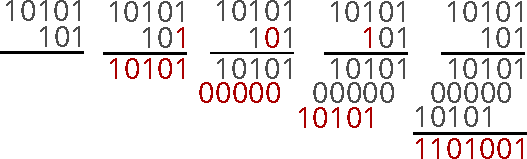
\includegraphics[width=0.5\textwidth]{binary_multiplication}
    \caption{Ukázka postupu násobení 0b010101 $\cdot{}$ 0b0101}\label{fig:binary_multiplication}
\end{figure}

Celočíselné dělení (\verb|mpt_div|) řešíme následovně:
\begin{enumerate}
    \item Najdeme v dělenci část (s nejvyšší vahou), od které lze odečíst dělitel
    \item Ve výsledné hodnotě nastavíme bit na pozici odpovídající LSB nalezené části na jedničku. Od nalezené části dělitel odečteme, a se vzniklým rozdílem pokračujeme
    \item Pokud jsme na konci dělence, algoritmus končí a výslednou hodnotu vrátíme
    \item K rozdílu přidáváme další bity dokud opět nemůžeme odečíst dělitel, poté se vrátíme ke kroku 2 
\end{enumerate}

Tento postup neprovádíme přímo se zadanými operandy, ale s jejich absolutními hodnotami, a pokud má být výsledná hodnota záporná, vrátíme na konci číslo opačné.

Postup dělení je ilustrován na obrázku~\ref{fig:binary_division}.

\begin{figure}[ht]
    \centering
    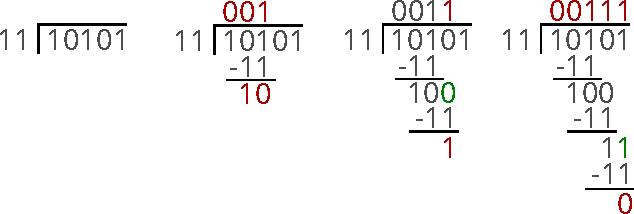
\includegraphics[width=0.5\textwidth]{binary_division}
    \caption{Ukázka postupu dělení 0b010101\textdiv0b011}\label{fig:binary_division}
\end{figure}
\newpage

Mocnění základu exponentem má v binární soustavě elegantní řešení~\cite{bib:power} popsané pseudokódem~\ref{alg:power}.

\begin{algorithm}[H]
\floatname{algorithm}{Algoritmus}
\caption{Umocnění základu exponentem v binární soustavě}\label{alg:power}
\begin{algorithmic}[1]
\scriptsize{
\Function{Power}{$base, exponent$}
	\If{$exponent = 0$}
		\State{\Return{$0$}}
	\EndIf{}
    \If{$exponent = 1$}
		\State{\Return{$base$}}
	\EndIf{}
    \State{$x:=base$}
    \For{$1$..bit\_count($exponent$)}
        \State{$x:=x^2$}
        \If{get\_bit($exponent$, bit\_count($exponent$)$ - i$)$ = 1$}
            \State{$x = x\cdot base$}
        \EndIf{}
    \EndFor{}
	\State{\Return{$x$}}
\EndFunction{}
}
\end{algorithmic}
\end{algorithm}

\subsection{Převod řetězce na MPT}
Funkce pro převody řetězců na \verb|mpt| se nachází v souborech \\ \verb|multiple_precision_parsing.c/.h|.

Pro převod používáme hlavně funkci \verb|mpt_parse_str|, která dokáže rozpoznat v jaké soustavě bylo číslo zadáné podle prefixu (\verb|0b / 0x|) nebo jeho absence. Funkce převádí číslo dokud jsou znaky pro danou soustavu platné a ve chvíli, kdy narazí na znak, který není součástí dané soustavy, ukončí činnost a vrátí hodnotu, kterou se podařilo převést. Během procházení znaků také mění ukazatel zadaný v parametru a na konci převodu bude ukazatel ukazovat na poslední znak, který číslu náležel.

Převod z čísel zadaných v binární soustavě probíhá následovně:
\begin{enumerate}
    \item Vytvoříme instanci \verb|mpt| s názvem \verb|new| a hodnotou 0
    \item Přečteme znak, a pokud nepatří do binární soustavy, ukončíme převod, jinak pokračujeme
    \item Hodnotu \verb|new| bitově posuneme o jednu pozici vlevo
    \item Nastavíme nultý bit \verb|new| na 1 nebo 0 podle aktuálního znaku
    \item Změníme ukazatel na další znak a vrátíme se na krok 2
\end{enumerate}
Převod z čísel zadaných v hexadecimální soustavě probíhá analogicky k binární soustavě s tím rozdílem, že bitový posun vlevo provádíme o čtyři pozice a místo nastavování nultého bitu, přičítáme hodnotu hexadecimálního znaku.

U těchto soustav musíme navíc ještě ošetřit, jestli byla čísla zadána v dvojkovém doplňku a mají být záporná. Např.~\verb|0b1101| by takto bylo převedeno na \verb|0b00001101| a je tedy třeba nastavit potřebné bity zleva na jedničku, k čemuž slouží statická funkce \verb|fill_set_bits_|.

Pro převod z dekadické soustavy používáme následující postup:
\begin{enumerate}
    \item Vytvoříme instanci \verb|mpt| s názvem \verb|new| a hodnotou 0
    \item Přečteme znak, a pokud nepatří do dekadické soustavy, ukončíme převod, jinak pokračujeme
    \item Hodnotu \verb|new| vynásobíme deseti
    \item K \verb|new| přičteme hodnotu znaku v dekadické soustavě.
    \item Změníme ukazatel na další znak a vrátíme se na krok 2
\end{enumerate}

\subsection{Výpisy MPT}
Funkce pro výpisy hodnot \verb|mpt| se nachází v souborech \\ \verb|multiple_precision_printing.c/.h|.

Pro výpis používáme funkci \verb|mpt_print|, která hodnotu vypíše v požadované soustavě.
\\\\
Výpis v binární soustavě je nejjednodušší:
\begin{enumerate}
    \item Vypíšeme '0b' a hodnotu MSB
    \item Ignorujeme všechny bity před (s nižší vahou) MSB, které mají stejnou hodnotu jako MSB
    \item Zbytek bitů vypíšeme v pořadí od nejvyššího po nultý
\end{enumerate} 

Výpis v hexadecimální soustavě provádíme po nibblech (čtveřice bitů) od nejvyššího nibblu po nultý.
\begin{enumerate}
    \item Vypíšeme '0x'
    \item Ignorujeme všechny nibbly s hodnotu \verb|0xf| (když MSB $ = 1$) nebo \verb|0x0| (když MSB $ = 0$)
    \item Pokud MSB $ = 0$ a aktuální nibble $\geq 8$, vypíšeme '0', jinak další krok
    \item Pokud MSB $ = 1$ a aktuální nibble $<8$, vypíšeme '0', jinak další krok
    \item Zbytek nibblů vypíšeme v pořadí od nejvyššího po nultý
\end{enumerate}

Pro výpis v dekadické soustavě si nejprve vytvoříme absolutní hodnotu zadané instance \verb|mpt|. Tu postupně dělíme deseti, kde zbytek po dělení nám postupně dá jednotlivé číslice v dekadické podobě. Číslice takto ale získáváme pozpátku, proto je nejprve ukládáme do vektoru, jehož obsah nakonec pozpátku vypíšeme, ještě před vypsáním vektoru ale vypíšeme znak mínusu, pokud bylo původní číslo záporné.

\subsection{Operátory}
Podporované operátory a k nim přidružené obslužné funkce, precedence a asociativity jsou ve struktuře \verb|func_oper_type| v souborech \verb|operators.c/.h|, spolu s funkcí \verb|get_func_operator| pro získání struktury \verb|func_oper_type| s daty, odpovídajícími požadovanému znaku operátoru.
\newpage

\subsection{Shunting yard}
Funkce pro zpracování zadaných výrazů se nachází v souborech \verb|shunting_yard.c/.h|.

Shunting yard je implementován standardně podle článku~\cite{bib:shunting_yard} a jeho činnost voláme funkcí \verb|shunt| s tím, že po úspěšném provedení algoritmu nejsou čísla ve výsledné RPN formě zapsána přímo, ale jsou reprezentována znakem 'n' a jejich skutečné \verb|mpt| hodnoty jsou uloženy ve výsledném zásobníku \verb|values|. Při vyhodnocování RPN pak při každém přečtení znaku 'n' skutečnou hodnotu čísla z tohoto zásobníku odebereme. 

Existuje speciální případ infixové formy, kde se, i přes správnou precedenci a asociativitu (podle tab.~\ref{tab:function}), RPN forma vytvoří v nesprávném tvaru, a to umocnění základu zápornou hodnotou např.~ve tvaru '\verb|4^-2|'. Správná forma RPN by byla '\verb|42-^|', s naším algoritmem by ale výsledná RPN forma byla '\verb|4^2-|', která by při vyhodnocování výsledku vrátila chybu. Z toho důvodu je tento speciální případ ošetřen ve statické funkci \verb|shunt_minus_| tak, že se operátor mínusu vynechá, zpracuje se výraz za mínusem a mínus se přidá do výsledné RPN formy naposled.

\begin{figure}[ht]
    \centering 
    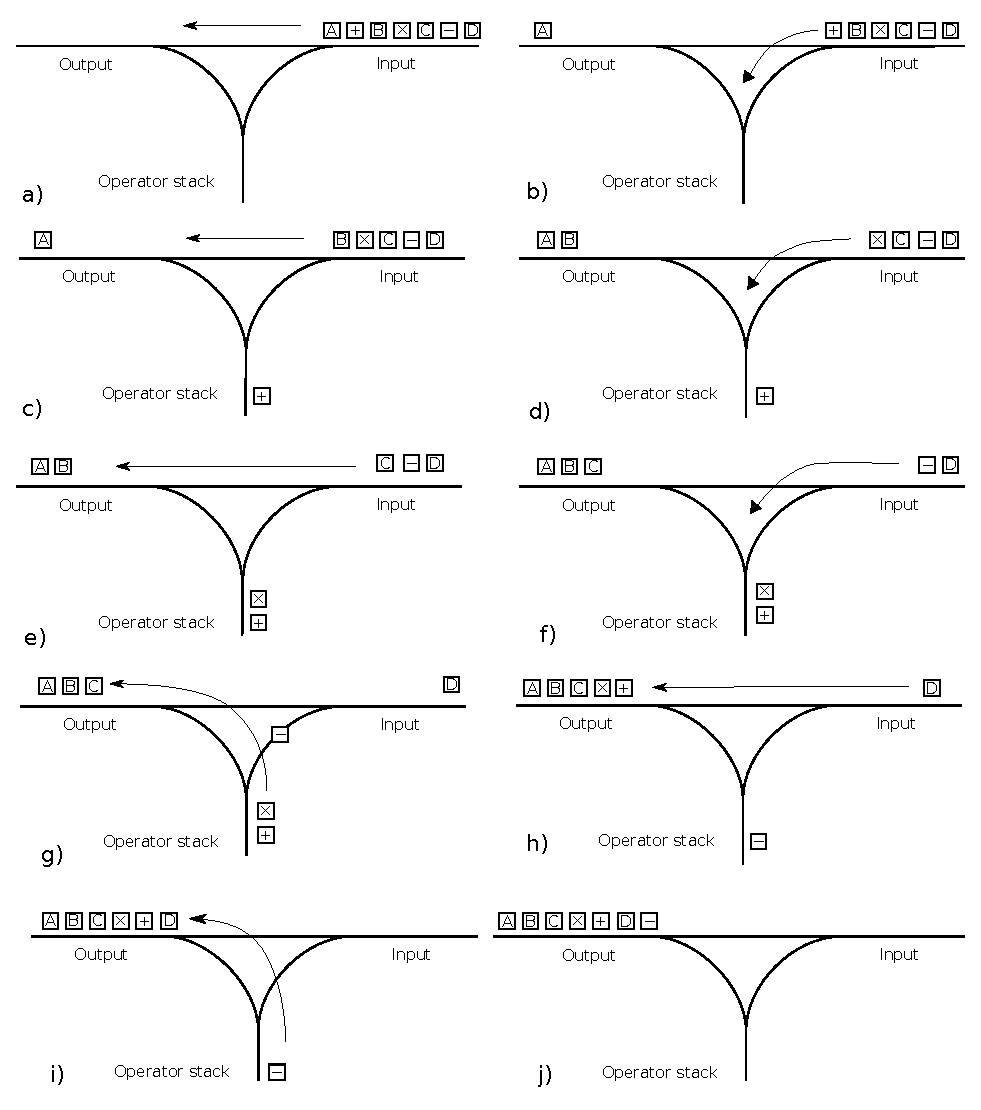
\includegraphics[width=0.8\textwidth]{shunting_yard}
    \caption{Ilustrace postupu algoritmu Shunting yard (převzato z~\cite{bib:shunting_yard}).}\label{fig:shunting_yard}
\end{figure}

\subsection{Vyhodnocení RPN}
Funkce pro vyhodnocení RPN se nachází v souborech \verb|shunting_yard.c/.h|.

Vyhodnocení výrazů ve formě RPN je také implementováno standardně. V algoritmu se využívá zásobník \verb|stack_values| pro mezivýsledky. Znaky výrazu zpracováváme jeden po druhém. Pokud narazíme na znak 'n', do \verb|stack_values| vložíme hodnotu \verb|mpt| odebranou ze zásobníku \verb|values|. Pokud je znak operátor, provedeme odpovídající operaci nad hodnotou, resp.~hodnotami odstraněnými ze zásobníku \verb|stack_values| a výsledek do stejného zásobníku vložíme.

Na konci vyhodnocení by se v zásobníku \verb|stack_values| měla nacházet jediná (výsledná) hodnota, a pokud tomu tak není, obsahoval výraz syntaktickou chybu.